% Bagian Tugas Pendahuluan
\section*{Tugas Pendahuluan}
\begin{enumerate}
  \item Install Visual Studio Code
  \begin{figure}[H]
    \centering
    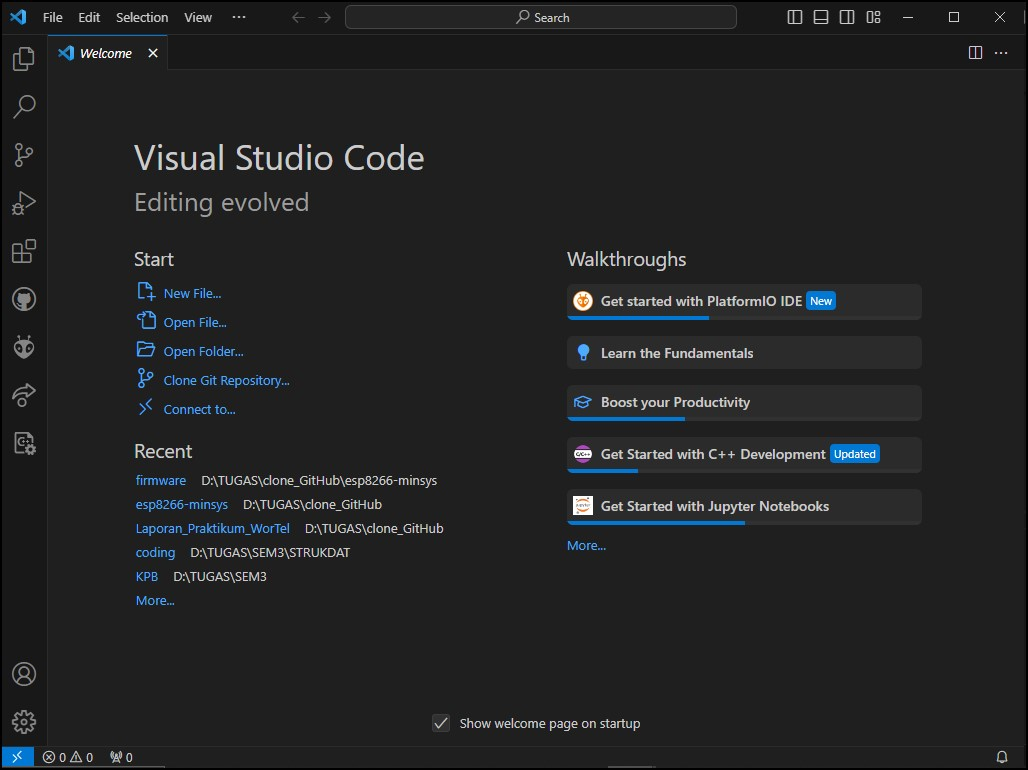
\includegraphics[width=0.6\linewidth]{img/modul_4/tupen_install_vscode.jpg}
    \caption{Bukti install VS Code} 
  \end{figure}
  \item Install ekstensi PlatformIO pada Visual Studio Code
  \begin{figure}[H]
    % Kalau mau menambah gambar lagi tinggal nambahin begin{subfigure} -> end{subfigure}
    \centering
    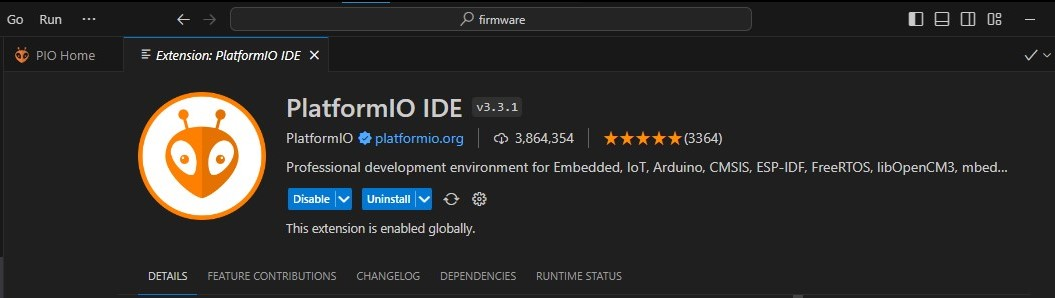
\includegraphics[width=0.9\linewidth]{img/modul_4/tupen_install_platformIO.jpg}
    \caption{Bukti install ekstensi PlatformIO \label{fig:inisub1}}
  \end{figure}
  \item Download firmware dari https://its.id/m/wortel-firmware lalu build project menggunakan vscode + Platformio sampai sukses
  \begin{figure}[H]
    \centering
    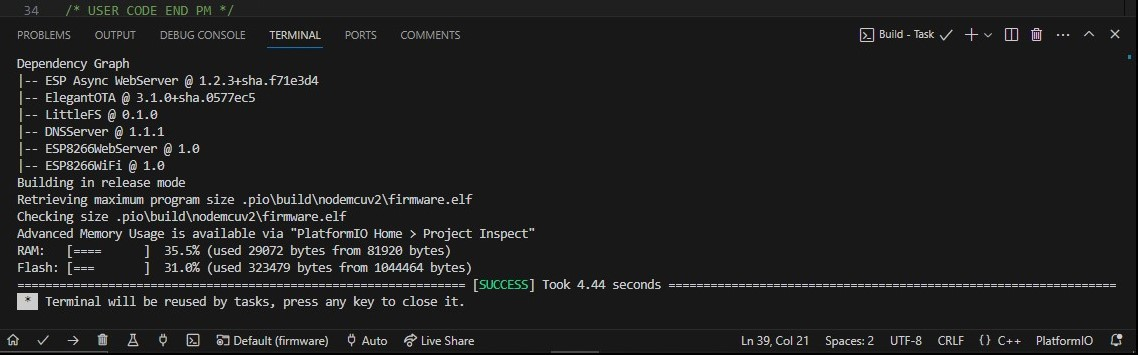
\includegraphics[width=0.9\linewidth]{img/modul_4/tupen_build_platformIO.jpg}
    \caption{Bukti sukses build project dengan platformIO \label{fig:inisub1}}
  \end{figure}
  \item Bukalah https://its.id/m/wortel-simulasi berikut lalu buat program untuk menghidupkan lampu ketika tombol ditekan

  \begin{lstlisting}[language=C++, caption= Kode yang disimulasikan]
  #define LED_RED 5
  #define LED_GREEN 16
  #define LED_BLUE 17
  #define BUTTON_ 26

  uint8_t led_color_rgb[3]={13 + 128, 13 * 2 + 38, 13 * 3 + 47};

  uint8_t btn_val = 0;

  void set_led_color(){
    analogWrite(LED_RED,led_color_rgb[0]);
    analogWrite(LED_GREEN,led_color_rgb[1]);
    analogWrite(LED_BLUE,led_color_rgb[2]);
  }

  void reset_led_color(){
    analogWrite(LED_RED,0);
    analogWrite(LED_GREEN,0);
    analogWrite(LED_BLUE,0);
  }

  void setup() {
    pinMode(LED_RED, OUTPUT);
    pinMode(LED_GREEN, OUTPUT);
    pinMode(LED_BLUE, OUTPUT);

    pinMode(BUTTON_, INPUT);
  }

  void loop() {
    btn_val = digitalRead(BUTTON_);

    if (btn_val == HIGH) {  // kalo tombol ditekan
      set_led_color();      // Atur warna lampu sesuai nilai yang udah ditentuin
    } else {                // kalo ga ditekan, reset warna lampu
      reset_led_color();
    }

    delay(10); 
  }
  \end{lstlisting}
  
  \begin{figure}[H]
    \centering
    % Kalau mau menambah gambar lagi tinggal nambahin begin{subfigure} -> end{subfigure}
    \begin{subfigure}[c]{0.46\linewidth}
      \centering
      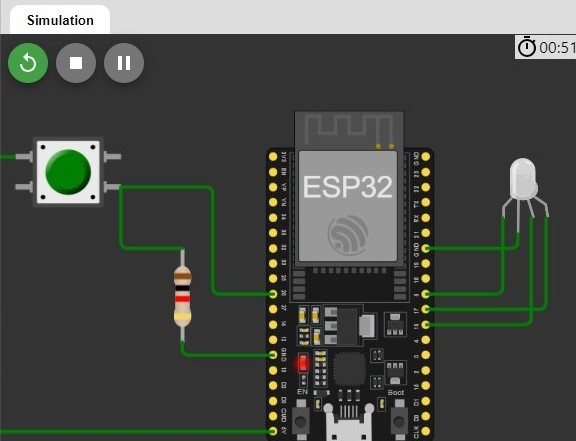
\includegraphics[width=\linewidth]{img/modul_4/tupen_lampu_mati.jpg}
      \caption{Simulasi saat button tidak ditekan (lampu reset) \label{fig:inisub1}}
    \end{subfigure}
    \hspace{1cm}
    \begin{subfigure}[c]{0.46\linewidth}
      \centering
      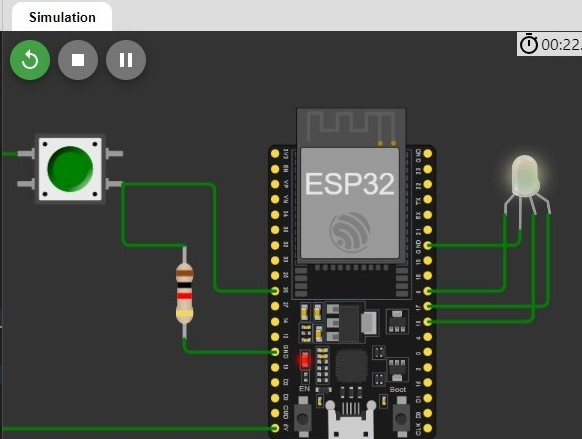
\includegraphics[width=\linewidth]{img/modul_4/tupen_lampu_nyala.jpg}
      \caption{Simulasi saat button ditekan (lampu nyala) \label{fig:inisub2}}
    \end{subfigure}
    \caption{Hasil simulasi \label{fig:keduagambar}}
  \end{figure}
\end{enumerate}
  

